\section{Introduktion}

\begin{frame}{Idé}%TODO: rename
\begin{center}
Kan man med \textbf{information} om trafiksignaler og evt. trængsel\\\textbf{spare brændstof} for den enkelte bil\\uden \textbf{nævneværdig negativ påvirkning} af anden trafik?
\end{center}
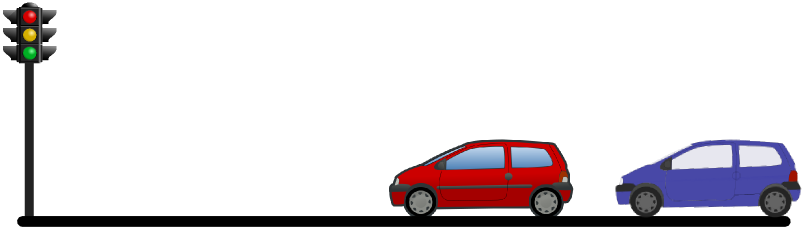
\includegraphics[width=1\textwidth]{../images/idea.png}
\end{frame}

\begin{frame}{Hvad er problemet?}
\textbf{Reducere brændsstofforbug} (miljø og økonomi)

\textbf{Maksimering af trafikflow}

Øge trafiksikkerhed

\vspace{5mm}
\begin{columns}%TODO: Align columns
\begin{column}{0.5\textwidth}
Muligheder
\begin{itemize}
\item Brændstofbesparende kørsel
\item \textbf{Minimere acceleration}
\item \textbf{Undgå fuld stop}
\end{itemize}

\end{column}
\begin{column}{0.4\textwidth}
Forhindinger
\begin{itemize}
\item Anden trafik
\item \textbf{Trafiklys}
\end{itemize}
\end{column}
\end{columns}
\end{frame}

\begin{frame}{Trafiklys}
Minimering af acceleration ved trafiklys og undgå fuld stop
\begin{itemize}
\item Adaptive trafiklys
\item \textbf{Tilpasse bilers hastighed til trafiklysene}
\end{itemize}


\begin{center}
\begin{columns}%TODO: Align columns
\begin{column}{0.4\textwidth}
Fordele
\begin{itemize}
\item Ingen ombygning af eksisterende lys
\item Virker ved lav penetrationsrate
\item Få invisteringsudgifter 
\end{itemize}
\end{column}

\begin{column}{0.5\textwidth}
Ulemper
\begin{itemize}
\item Kræver biler løbende kan aflæse trafiksignaler
\item Påvirkning af øvrig trafik?
\item Overholde hastighedsbegrænsinger %TODO: omformuler. Det at folk kan se at de kan nå lyset, hvis de køre forstærkt.
\end{itemize}
\vspace{8mm}
\end{column}
\end{columns}
\end{center}
\end{frame}

\begin{frame}{Hastighedstilpasning}
\begin{columns}
\begin{column}{0.4\textwidth}
\begin{itemize}
\item Et tænkt lyskryds
\item Minimim 15 km/t
\end{itemize}
\end{column}
\begin{column}{0.6\textwidth}
\begin{itemize}
\item Blå biler: uden \tech
\item Røde biler: med \tech
\end{itemize}
\end{column}
\end{columns}

\vspace{3mm}
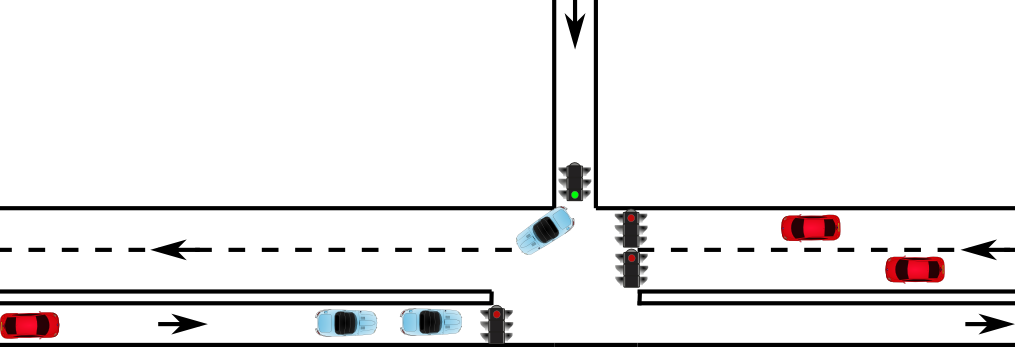
\includegraphics[width=1\textwidth]{../images/introNetworkSimple.png}
\end{frame}

\begin{frame}{Hastighedstilpasning}
\begin{columns}
\begin{column}{0.4\textwidth}
\begin{itemize}
\item Et tænkt lyskryds
\item Minimim 15 km/t
\end{itemize}
\end{column}
\begin{column}{0.6\textwidth}
\begin{itemize}
\item Blå biler: uden GreenFlow
\item Røde biler: med GreenFlow
\end{itemize}
\end{column}
\end{columns}
\vspace{3mm}
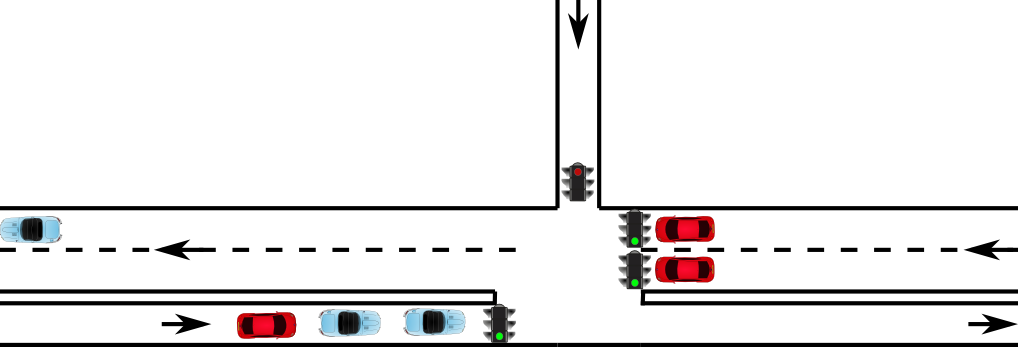
\includegraphics[width=1\textwidth]{../images/introNetworkSimple2.png}
\end{frame}

\begin{frame}{Vision}
\begin{center}
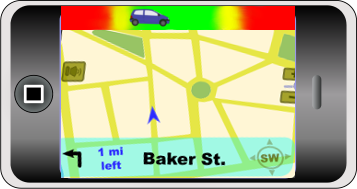
\includegraphics[width=1\textwidth]{../images/product.png}
\end{center}
\end{frame}
